\section{Introduzione}


\begin{frame}
    \frametitle{Morteratsch in numeri}
    \framesubtitle{}

    \begin{columns}
        \begin{column}{0.5\textwidth}
            \begin{itemize}[itemsep=0.5em, label=$\bullet$]
                \item Superficie: 14.93 km$^2$
                \item Volume: 0.899 km$^3$
                \item Quota fronte: 2117 m
                \item Quota massima: 4049 m
                \item Spessore medio: 61.4 m
                \item Spessore massimo: 280.7 m
            \end{itemize}
            \vspace{12pt}

            Dati da \hypercite{https://doi.glamos.ch/pubs/glrep/glrep_141-142.html}{GLAMOS22}
        \end{column}
        
        \begin{column}{0.5\textwidth}
        \begin{figure}
            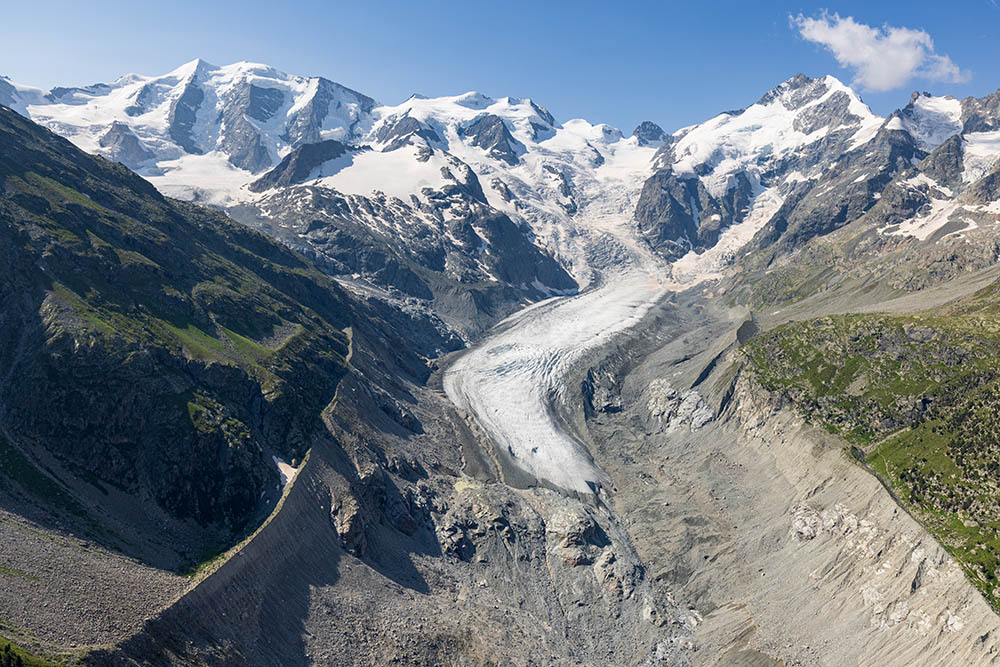
\includegraphics[width=0.8\textwidth]{Immagini/AereaMorteratsch.jpg}
            \caption{Foto da \href{https://www.swisseduc.ch/glaciers/morteratsch/2021/index-en.html}{\textcolor{blue}{SwissEduc}}}
          \end{figure}
        \end{column}
      \end{columns}
  
\end{frame}


\begin{frame}
  \frametitle{Confronto}
  \framesubtitle{}
  
  \begin{figure}
    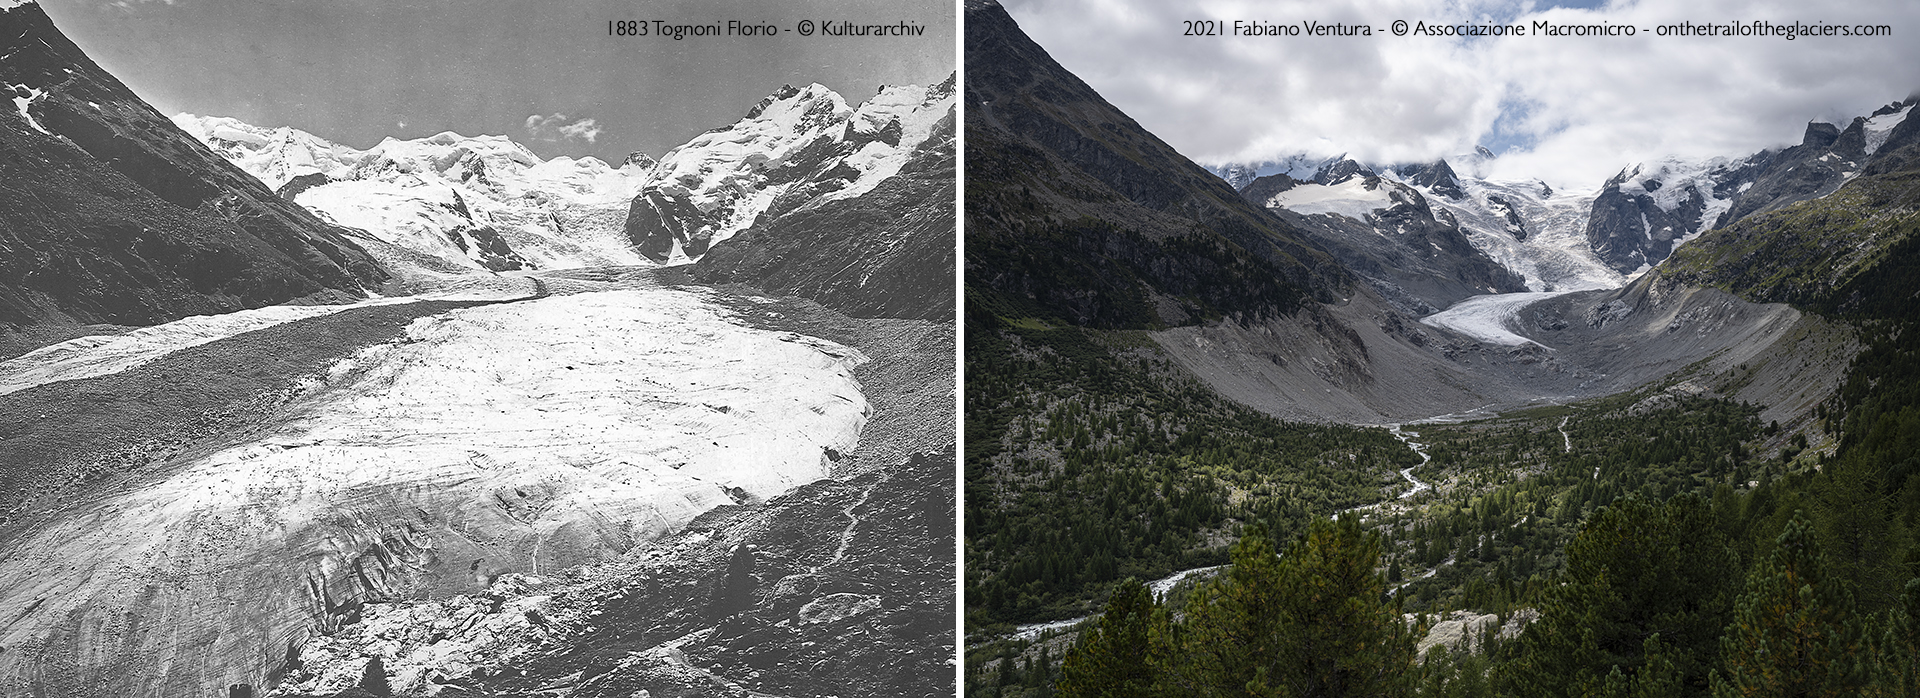
\includegraphics[width=\textwidth]{Immagini/ConfrontoMorteratsch.jpg}
    \caption{Ghiacciaio del Morteratsch nel 1883 e nel 2021. (Fabiano Ventura - 2021)}
  \end{figure}

\end{frame}

\begin{frame}
  \frametitle{Vadret Pers}
  \framesubtitle{}

  \begin{columns}
      \begin{column}{0.5\textwidth}
          \begin{itemize}[itemsep=0.5em, label=$\bullet$]
              \item Separato dal Morteratsch nel 2017
              \item Superficie: 6.7 km$^2$
              \item Quota minima: 2450 m
              \item Quota massima: 3900 m
          \end{itemize}
          \vspace{12pt}

          Dati da \hypercite{https://doi.glamos.ch/pubs/glrep/glrep_141-142.html}{GLAMOS22}
      \end{column}
      
      \begin{column}{0.5\textwidth}
      \begin{figure}
          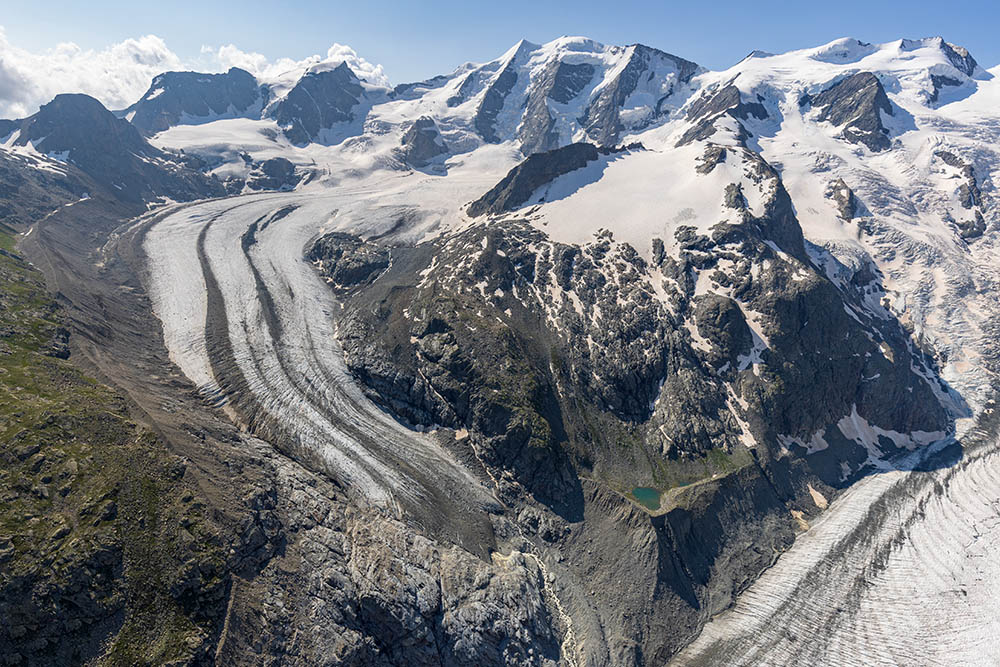
\includegraphics[width=0.8\textwidth]{Immagini/vadretPers.jpg}
          \caption{Foto da \href{https://www.swisseduc.ch/glaciers/morteratsch/2021/index-en.html}{\textcolor{blue}{SwissEduc}}}
        \end{figure}
      \end{column}
    \end{columns}

\end{frame}